\documentclass[a4paper]{article}
\title{Imitation Learning}
\author{Andrija Djurisic}
\date{July 2020}

\usepackage{mathtools}
\usepackage[export]{adjustbox}
\usepackage{amsmath}
\usepackage{amsthm}

\begin{document}
	\maketitle

Imitation learning is the umbrella term for family of Machine Learning methods where neural net attempts to learn from human demonstration.

\subsubsection*{Behavioral cloning}
Behavioral cloning treats imitation learning as a supervised learning problem. That is, it learns to map actions to states [\ref{fig:behavioral_cloning}] the same way a neural network competing in the ImageNet challenge learns to map labels to images. By doing that we are learning the policy $\pi_{\theta}(a_{t}|{o}_{t})$.

\begin{figure}[h]
	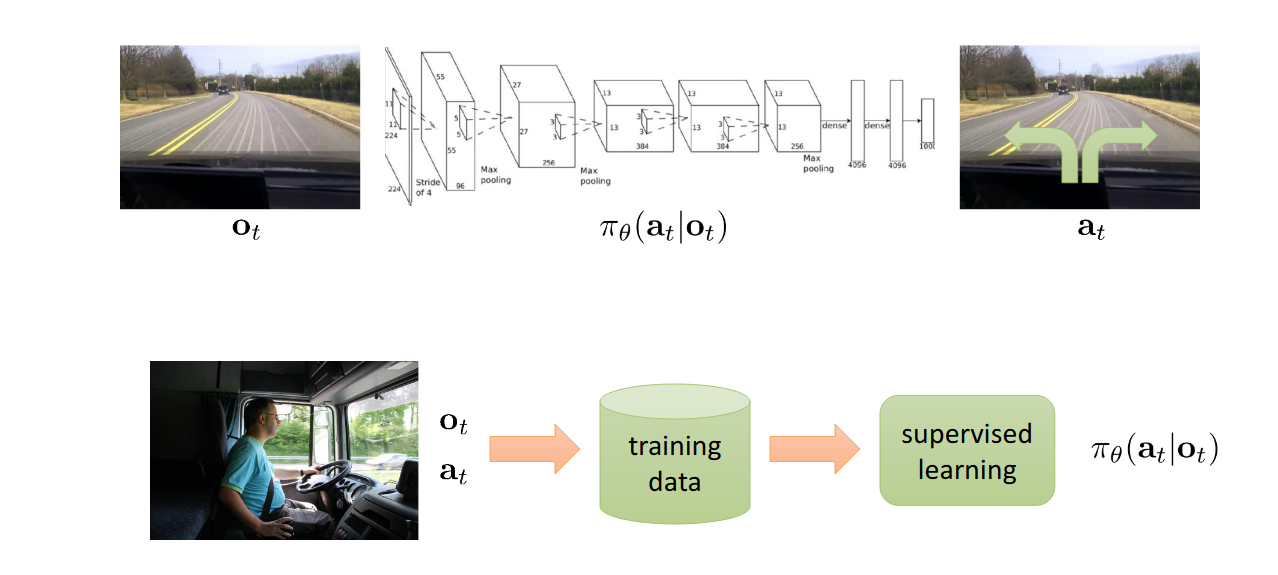
\includegraphics[width=\linewidth]{imgs_tex/bh.png}
	\caption{Behavioral cloning.}
	\label{fig:behavioral_cloning}
\end{figure}

The theoretical reason why behavioral cloning might not do so well is that when we fit our policy to training data, learned policy won't be perfect. It will occasionally make mistakes and those mistakes will gradually create a bigger and bigger drift [\ref{fig:drift}], thus putting the agent in the state with the properties that weren't encountered during the training.

\pagebreak

\begin{figure}[h]
	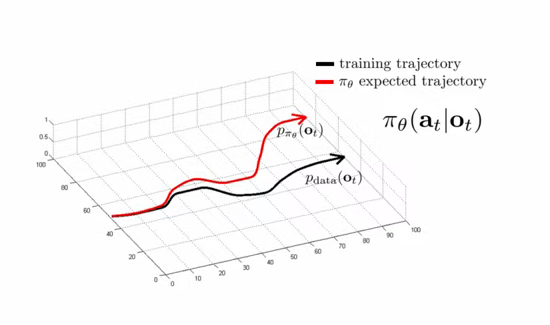
\includegraphics[width=0.7\textwidth, center]{imgs_tex/drift.png}
	\caption{Drift caused by accumulating mistakes due to imperfect policy.}
	\label{fig:drift}
\end{figure}


\subsubsection*{DAgger}

One way to get around the problem we described is to collect more data, especially in the areas where agent drifted away. The \textbf{D}ataset \textbf{A}ggregation is a four steps algorithm [\ref{fig:dagger}] that describes how to collect more data.

\begin{figure}[h]
	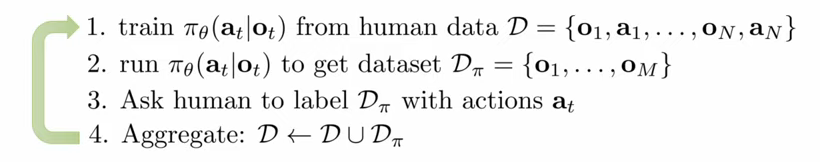
\includegraphics[width=0.7\textwidth, center]{imgs_tex/dagger.png}
	\caption{Dagger.}
	\label{fig:dagger}
\end{figure}


\subsubsection*{Theoretical evaluation of Behavioral cloning}

\begin{proof}
\end{proof}

\end{document}

